
\documentclass[12pt]{article}

\usepackage{/home/andreas/Templates/Packages}
\addbibresource{Ref.bib}

% GLOSSARY STUFF ------------------------------------
\makenoidxglossaries   % REQUIRED for noidx
%\makeglossary


% Define acronyms
\newabbreviation{sph}{SPH}{Smoothed Particle Hydronamics}
% ----------------------------------------------------

\begin{document}
	
\begin{titlepage}
	\begin{center}
		\includegraphics[height=5cm]{/home/andreas/Lund/Figures/LU_NaturVetFak_RGB_ENG.png}
		\vspace{5cm}
		
		{\Huge{\bf Differential Equations in Astrophysics}}\\
		\vspace{1cm}
		{\Large{\bf Andreas Pettersson}}\\
		\vspace{5mm}
		{\Large{\bf in Collaboration with Leo Bublies}}
		
	\end{center}
\end{titlepage}
	
\pagenumbering{roman} 

% GLOSSARY

\newpage
% Print the acronym list
\printnoidxglossary[type=abbreviations,style=list,title={List of Abbreviations}]

\newpage
\tableofcontents
\newpage
\setcounter{page}{1}
\pagenumbering{arabic} 

\section{Introduction}

\gls{sph} is an efficient way for simulating continuous systems, such as fluid dynamics. It is constructed in a meshfree grid of particles, where the interactions between nearest neighbours are determined by a smoothing kernel. The smoothing kernel itself is generally given as a cubic spline or occasionally as a Gaussian distribution; as the form of the kernel is dependent on the problem at hand, there is no universally accepted approach.\newline 
In this report the \gls{sph} method will be used to simulate Sod's shock tube and two gas-like planets colliding.\newline
Sod's shock tube is a widely used computational problem that is used to assert correctly written --- as well as the efficiency --- of written \gls{sph} code. Since the same set of main equations are used to simulate the two gas-like planets, Sod' shock tube problem is appropriately chosen to ascertain working code, as mentioned. 

\section{Theory}

Here the theory --- and mainly equations --- are given for each project; being Sod' shock tube and the collision of two gas-like planets. 

\subsection{Smoothing kernel}

The smoothing kernel, or simply kernel, is denoted $W(R,h)$. In the two simulations mentioned, the following form is used:
\begin{equation}
	W = \alpha_d\times
	\begin{cases}
		\frac{2}{3} - R^2 + \frac{1}{2}R^3, & 0\leq R < 1\\
		\frac{1}{6}(2-R)^3, & 1 \leq R < 2\\
		0, & R\geq 2
	\end{cases},
\end{equation}
where $R_{ij} = r_{ij}/h = \vert\mathbf{x}_i - \mathbf{x}_j\vert/h = \vert d\mathbf{x}\vert/h$, with $h$ being the smoothing length. In addition, the gradient of the kernel --- which is naturally used in the equations --- is given by 
\begin{equation}
	\nabla W(R,h) = 
	\begin{cases}
		\alpha_d\times \left(-2 + \frac{3}{2}R\right)\frac{d\mathbf{x}}{h^2}, & 0 \leq R < 1\\
		-\alpha_d\times \frac{1}{2}(2-R)^2\frac{d\mathbf{x}}{hr}, & 1\leq R < 2\\
		0, & R\geq 2
	\end{cases}.
\end{equation}
The quantity $\alpha_d$ is dependent on the dimension $d$ and is given by 
\begin{align}
	\alpha_1 &= \frac{1}{h}\\
	\alpha_2 &= \frac{15}{7\pi h^2}\\
	\alpha_3 &= \frac{3}{2\pi h^3}.
\end{align}

\subsection{Sod's Shock Tube}

Sod's shock tube is composed of a 1-dimensional 'tube' with particles spread out along the $x$-axis. A membrane is placed in the middle of the tube, where each side of the membrane contain a difference in particles and hence density and pressure. Using a summation density approach, the equations used stems from the Navier-Stokes equations, where the density for the $i$:th particle is given by 
\begin{equation}
	\rho_i = \sum_j m_jW_{ij}.
\end{equation}
Here $m_j$ is the mass of the $j$:th particle and $W_{ij}$ the smoothing kernel. Furthermore, the pressure is calculated by the equations of state;
\begin{equation}
	p_i = (\gamma - 1)\rho_ie_i,
\end{equation}
where $e_i$ is the energy and $\gamma = C_p/C_v = 1.4$ is the ratio between the heat capacity at constant pressure and volume. The rate of change of position is given by 
\begin{equation}
	\frac{d\mathbf{x}_i}{dt} = \mathbf{v}_i,
\end{equation}
$\mathbf{v}_i$ being the velocity. In turn, the rate of change of velocity is
\begin{equation}
	\frac{d\mathbf{v}_i}{dt} = -\sum_{j=1}^N m_j\left(\frac{p_i}{\rho_i^2} + \frac{p_j}{\rho_j^2} + \Pi_{ij}\right)\nabla_iW_{ij}.
\end{equation}
Here, the term $\Pi_{ij}$ is the artificial viscosity; if not added, un-physical results will occur. It is given by 
\begin{equation}
	\Pi_{ij} = 
	\begin{cases}
		\frac{-\alpha_\Pi\Bar{c}_{ij}\phi_{ij} + \beta_\Pi\phi_{ij}^2}{\Bar{\rho}_{ij}}, &\mathbf{v}_{ij}\cdot\mathbf{x}_{ij} < 0\\
		0 ,&\mathbf{v}_{ij}\cdot\mathbf{x}_{ij} \geq 0
	\end{cases}.
\end{equation}
The terms $\alpha_\Pi$, $\beta_\Pi$ are constants, while
\begin{equation}
	\phi_{ij} = \frac{h_{ij}\mathbf{v}_{ij}\cdot\mathbf{x}_{ij}}{\vert\mathbf{x}_{ij}\vert^2 + \varphi^2},
\end{equation}
where $\mathbf{x}_{ij} = \mathbf{x}_i - \mathbf{x}_j$ and similarly for $\mathbf{v}_{ij}$. Furthermore, $\varphi = 0.1h_{ij}$ and 
\begin{equation}
	\Bar{\rho}_{ij} = \frac{1}{2}(\rho_i + \rho_j),
\end{equation}
is the average density. Similarly, $\Bar{c}_{ij}$ is the average sound speed, where the sound speed is given by 
\begin{equation}
	c_i = \sqrt{(\gamma - 1)e_i},
\end{equation}
and $h_{ij}$ is the average smoothing length used in the kernel. Finally, the rate of change of energy is given by 
\begin{equation}
	\frac{de_i}{dt} = \frac{1}{2}\sum_{j=1}^N m_j\left(\frac{p_i}{\rho_i^2} + \frac{p_j}{\rho_j^2} + \Pi_{ij}\right)\mathbf{v}_{ij}\cdot\nabla_iW_{ij}.
\end{equation}

\subsection{Planet Collision}

For the two gas-like planets colliding, the same equations are implemented with the exception of gravity. Thus, in addition to the above stated equations, a gravitational acceleration is added, given by 
\begin{equation}
	\left(\frac{d\mathbf{v}_i}{dt}\right)_{\mathrm{Gravity}} = -\frac{G}{2}\sum_{j=1}^N m_j(\nabla_i\phi_{ij}(h_i) + \nabla_i\phi_{ij}(h_j))\frac{\mathbf{x}_{ij}}{r_{ij}},
\end{equation}
where $G$ is the gravitational constant and $\nabla\phi$ is the gradient of the gravitational potential, given by 
\begin{equation}
	\frac{\partial\phi(r,h)}{\partial r} = 
	\begin{cases}
		\frac{1}{h^2}(\frac{4}{3}R - \frac{6}{5}R^3 + \frac{1}{2}R^4), & 0 \leq R < 1\\
		\frac{1}{h^2}(\frac{8}{3}R - 3R^2 + \frac{6}{5}R^3 - \frac{1}{6}R^4 - \frac{1}{15R^2}, & 1\leq R < 2\\
		\frac{1}{r^2}, & R\geq2
	\end{cases}.
\end{equation}


\section{Method}

Both sub-projects were programmed in python using the numpy and scipy libraries. No for-loops were used, in favor of broadcasting numpy matrices. 

\subsection{Sod's Shock Tube}

For Sod's shock tube in 1-D, 400 particles were used, with initial conditions given in the lab manual\cite{Hobbs}. The smoothing constant $ h $ giving 5 nearest neighbors was found to be 0.01 through inspecting matrices, and was used throughout the simulations. The integrator used was RK45 with the scipy tool scipy.integrator.solve\_ivp.

\subsection{Planet Collision}

For planet collisions, 600 particles were used, with 300 per planet. The smoothing constant $ h $ was found to be $ 1 \cdot 10^7 $. The same integrator was used as in the 1-D problem.

\section{Results}

Here is presented the results from Sod's shock tube and planetary collisions.

\subsection{Sod's Shock Tube}

Running the simulation with $ dt = 0.05 $ and 20~steps, produced the results in \textbf{Fig~\ref{fig:1d}}.

\begin{figure}[H]
	\centering
	
	% Top-left
	\begin{subfigure}[c]{0.45\textwidth}
		\centering
		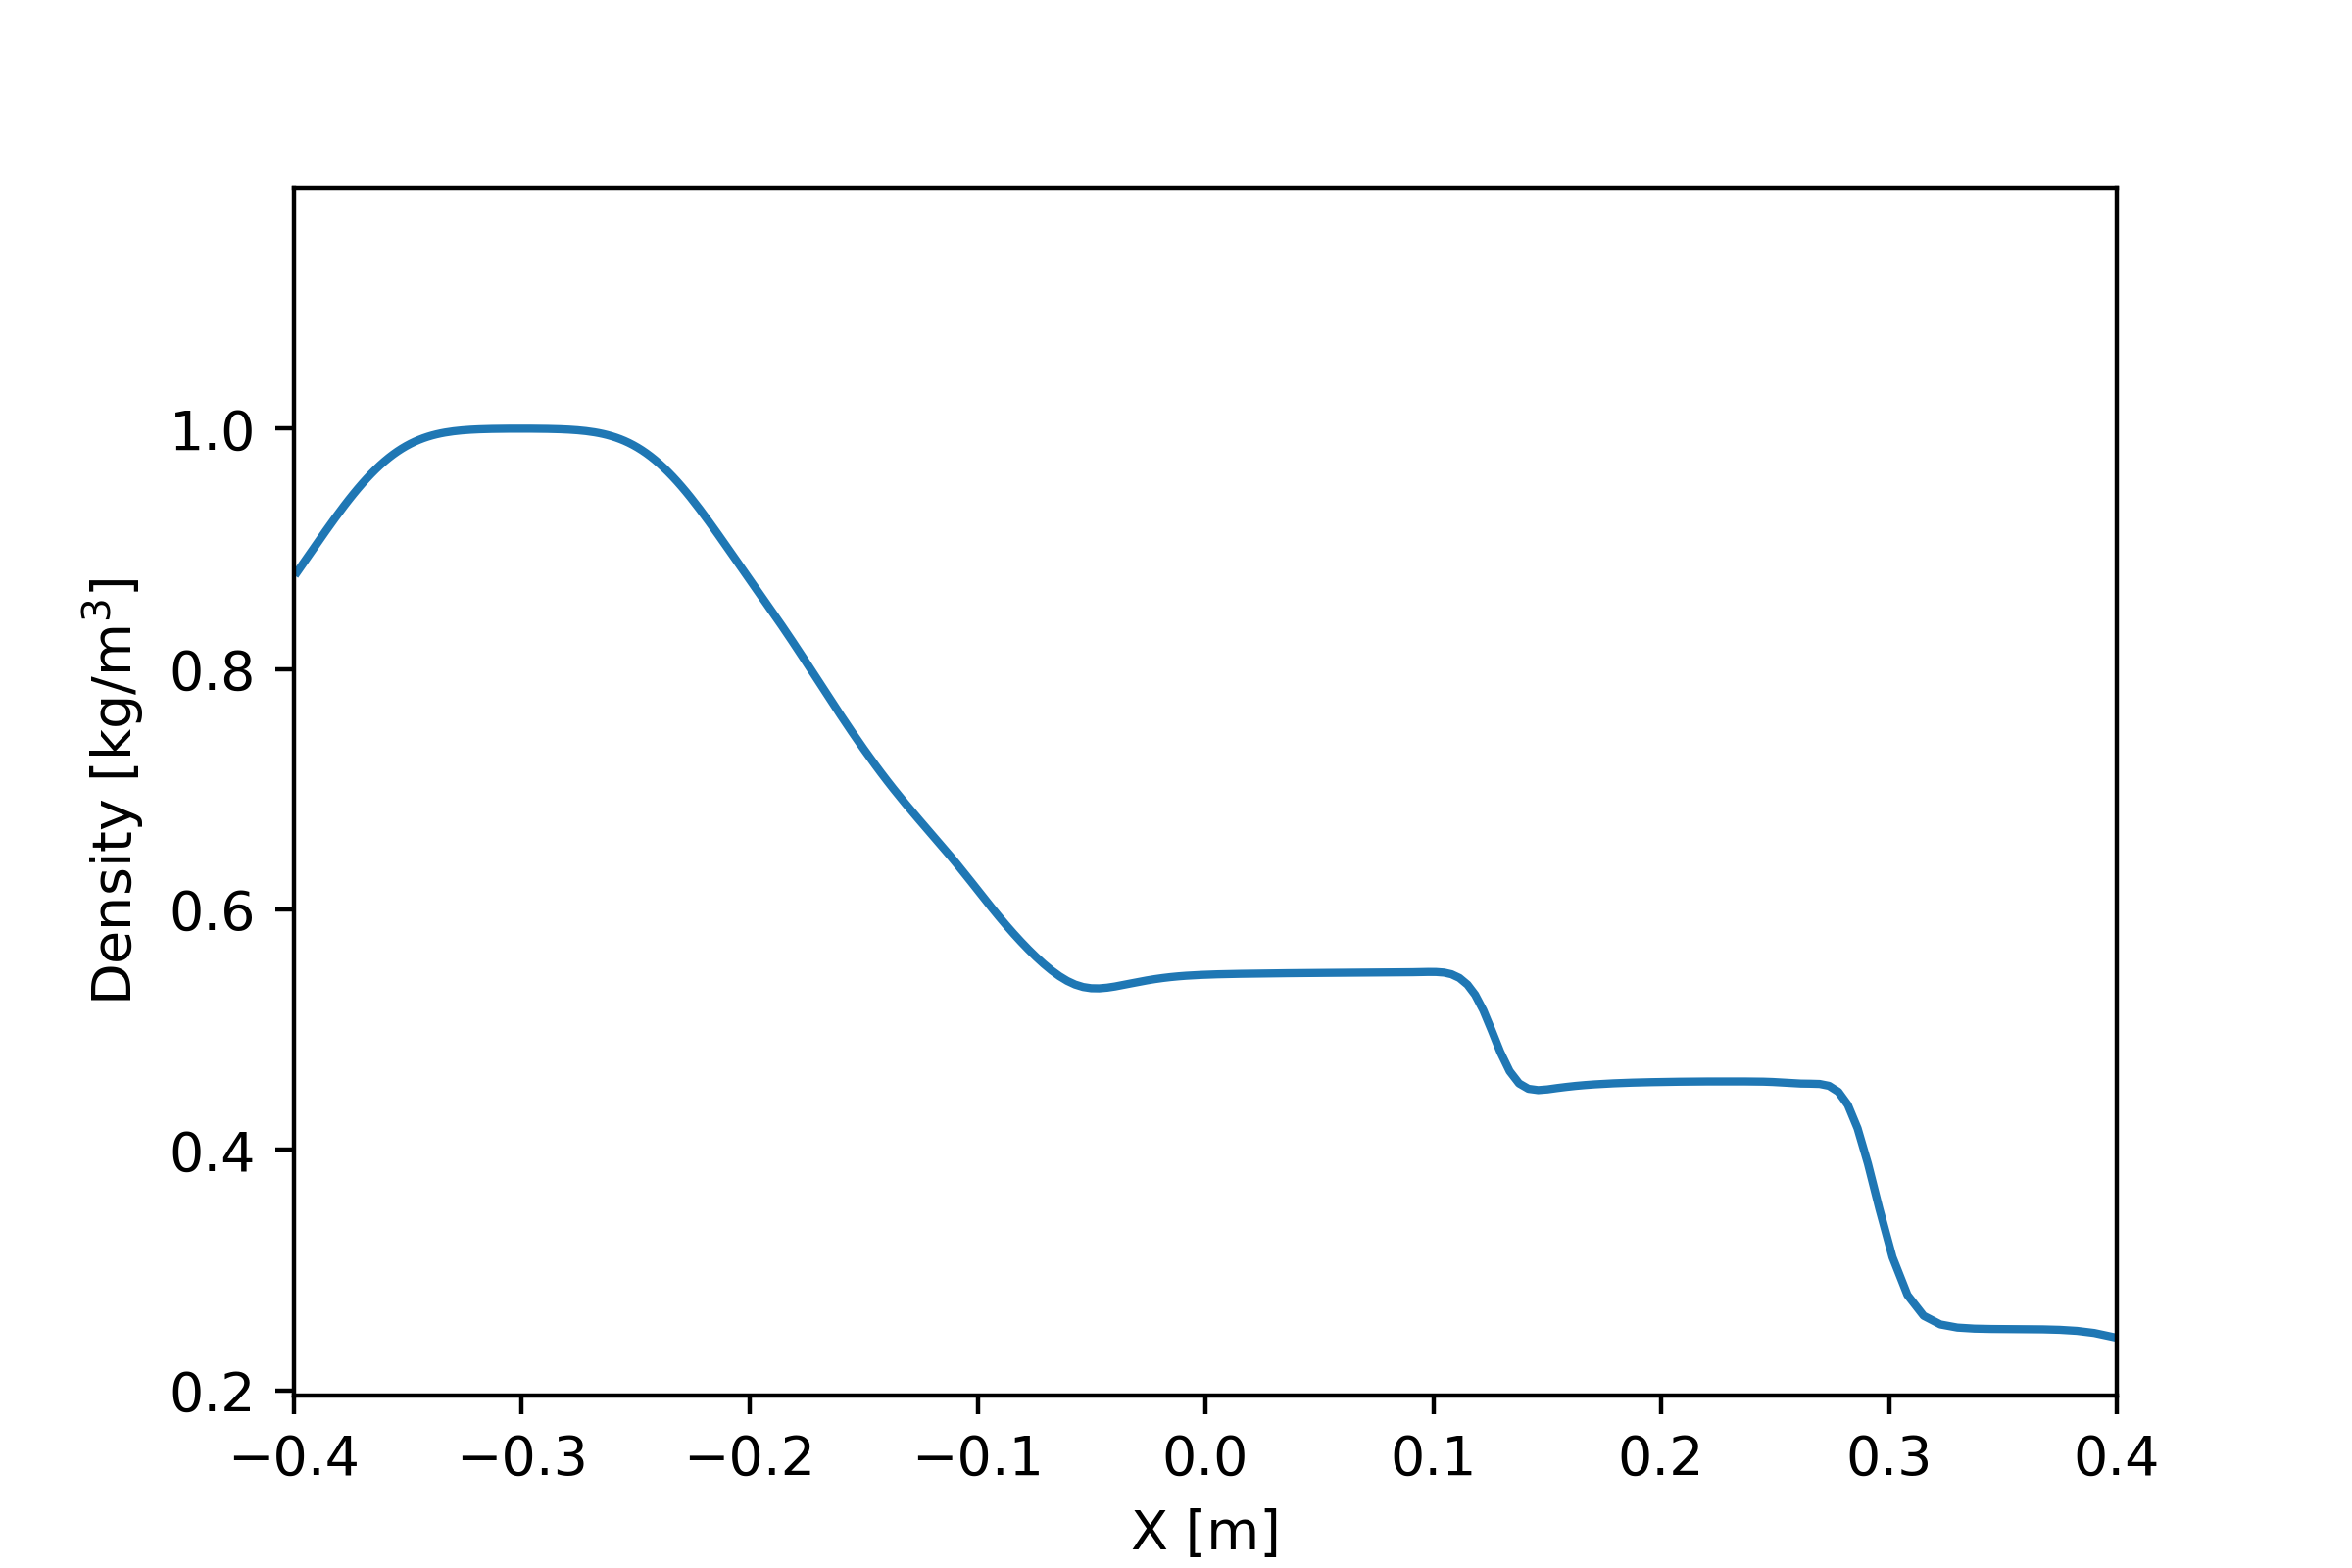
\includegraphics[width=\linewidth]{/home/andreas/Lund/FYSN33/Labs/SPH/SPH-Lab/1D/Density.png}
	\end{subfigure}
	\hfill
	% Top-right
	\begin{subfigure}[c]{0.45\textwidth}
		\centering
		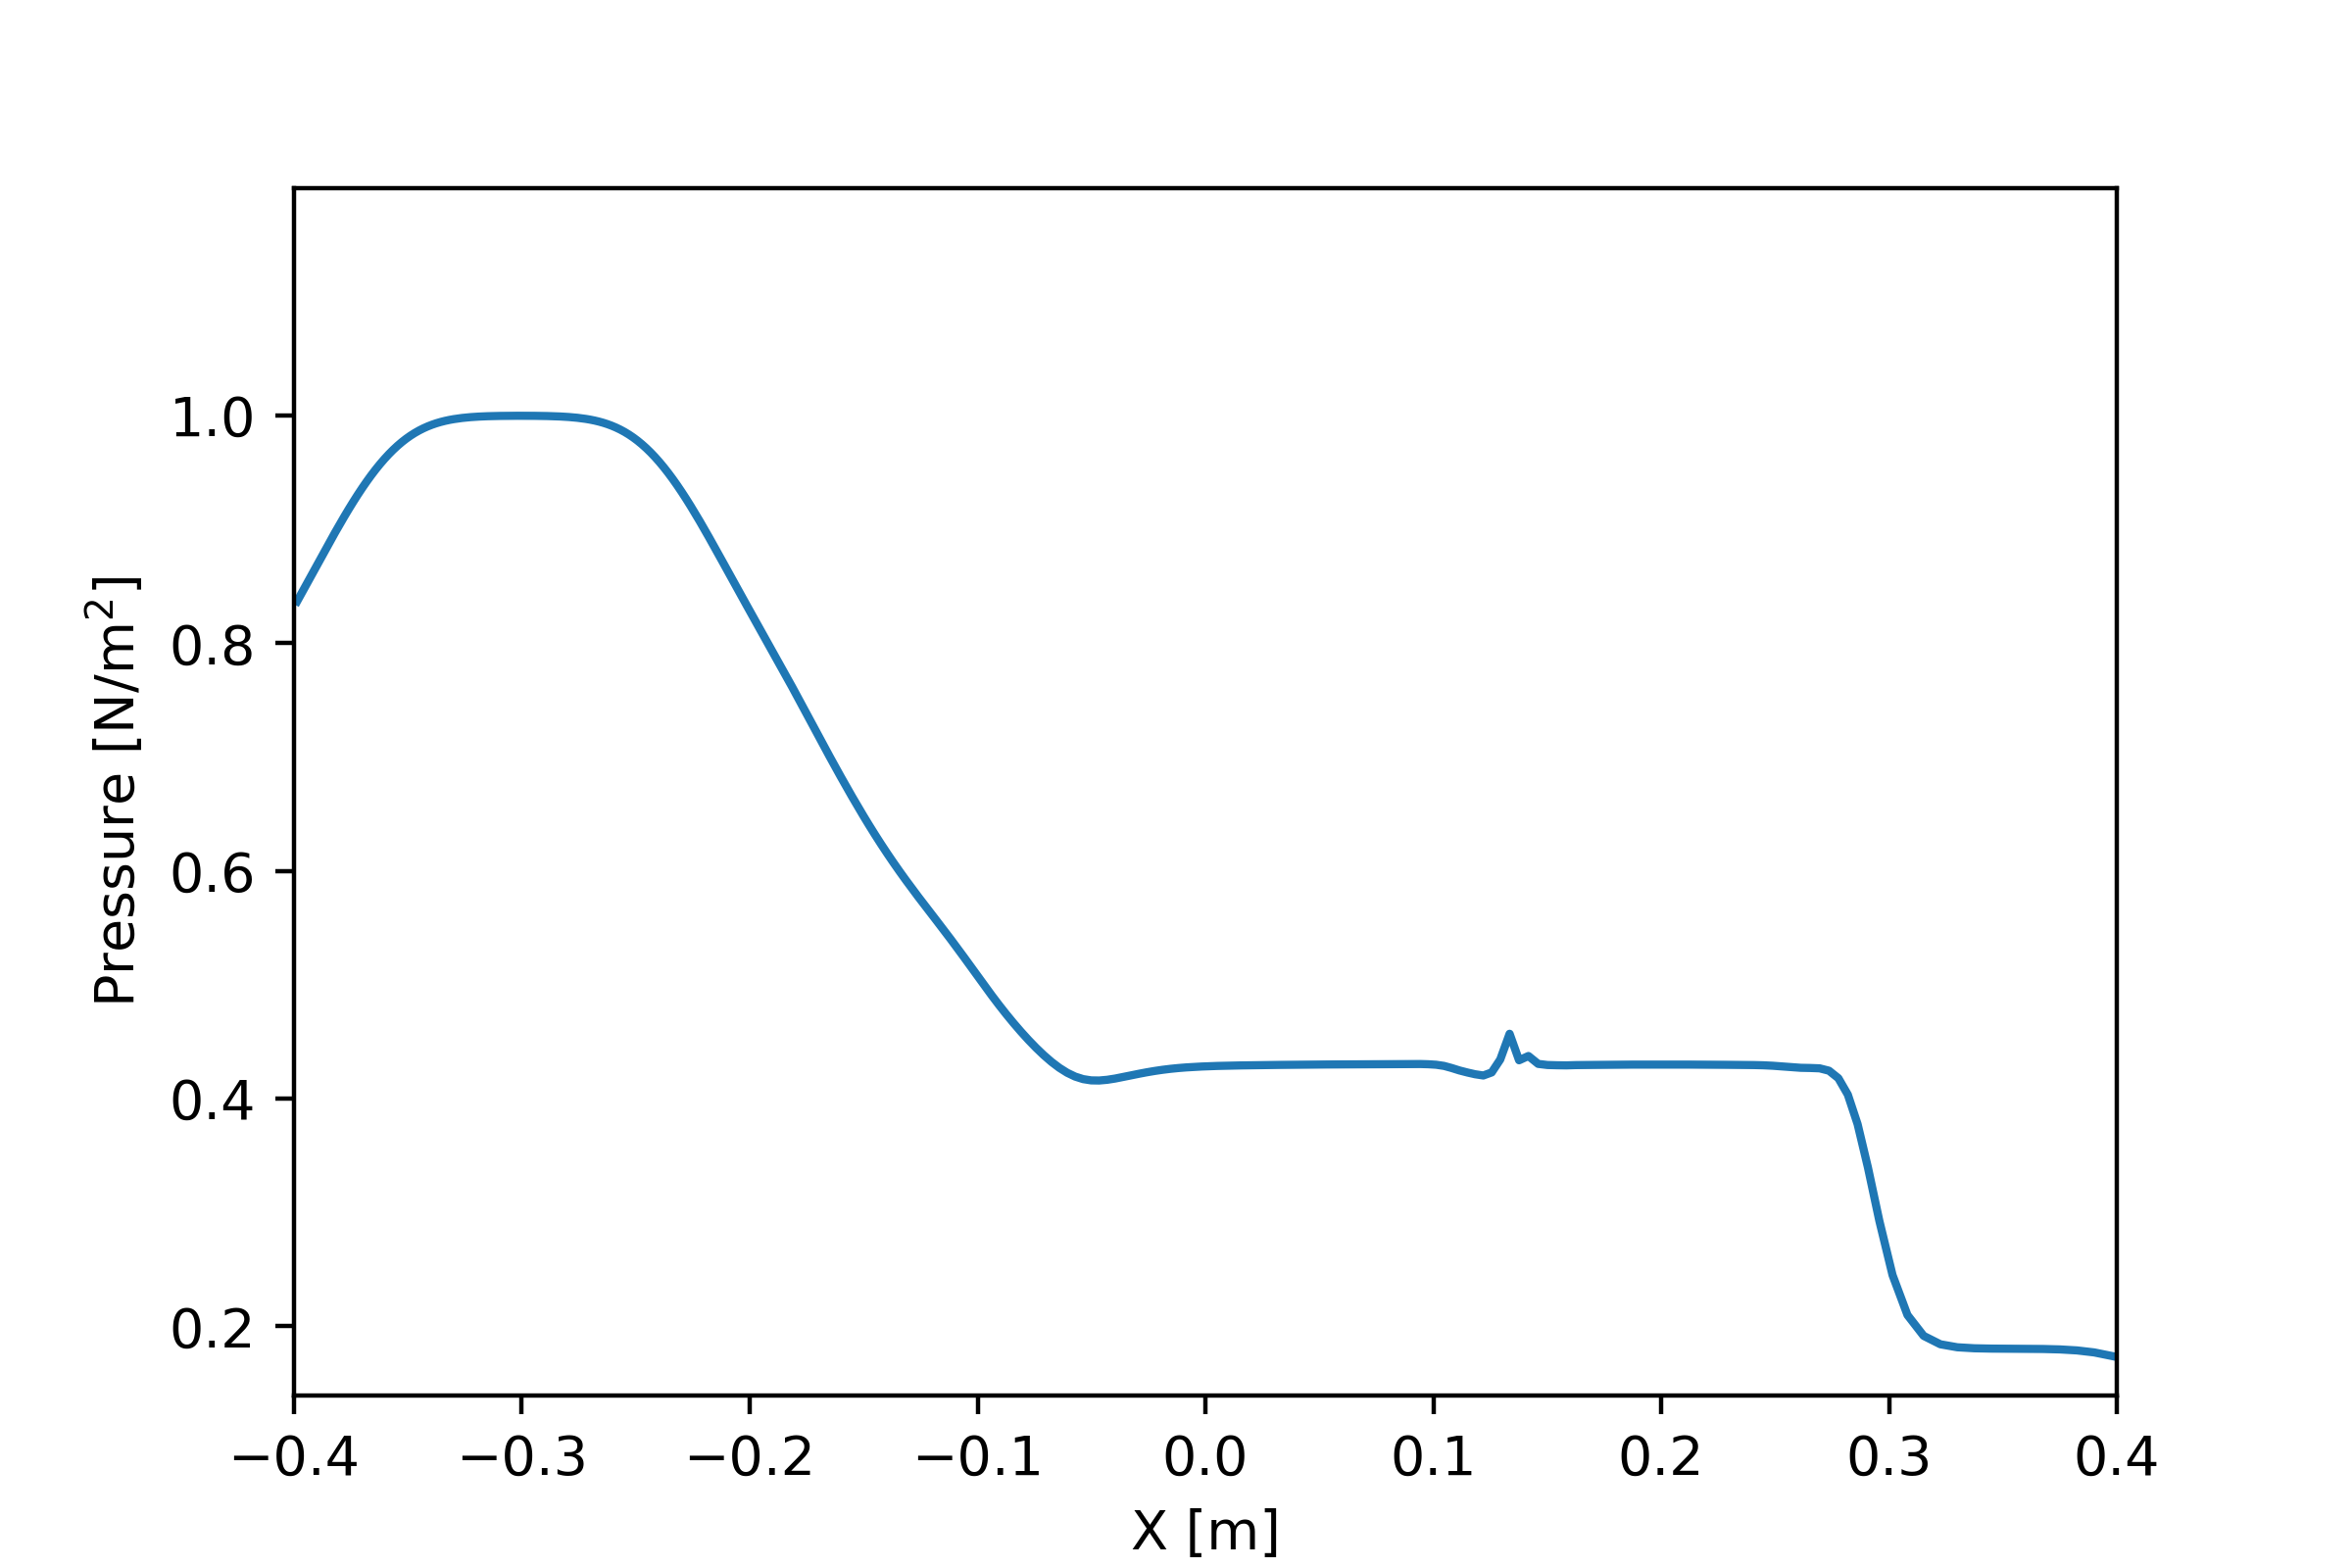
\includegraphics[width=\linewidth]{/home/andreas/Lund/FYSN33/Labs/SPH/SPH-Lab/1D/Pressure.png}
	\end{subfigure}
	
	\vskip 0.1cm % vertical spacing between rows
	
	% Bottom-left
	\begin{subfigure}[c]{0.45\textwidth}
		\centering
		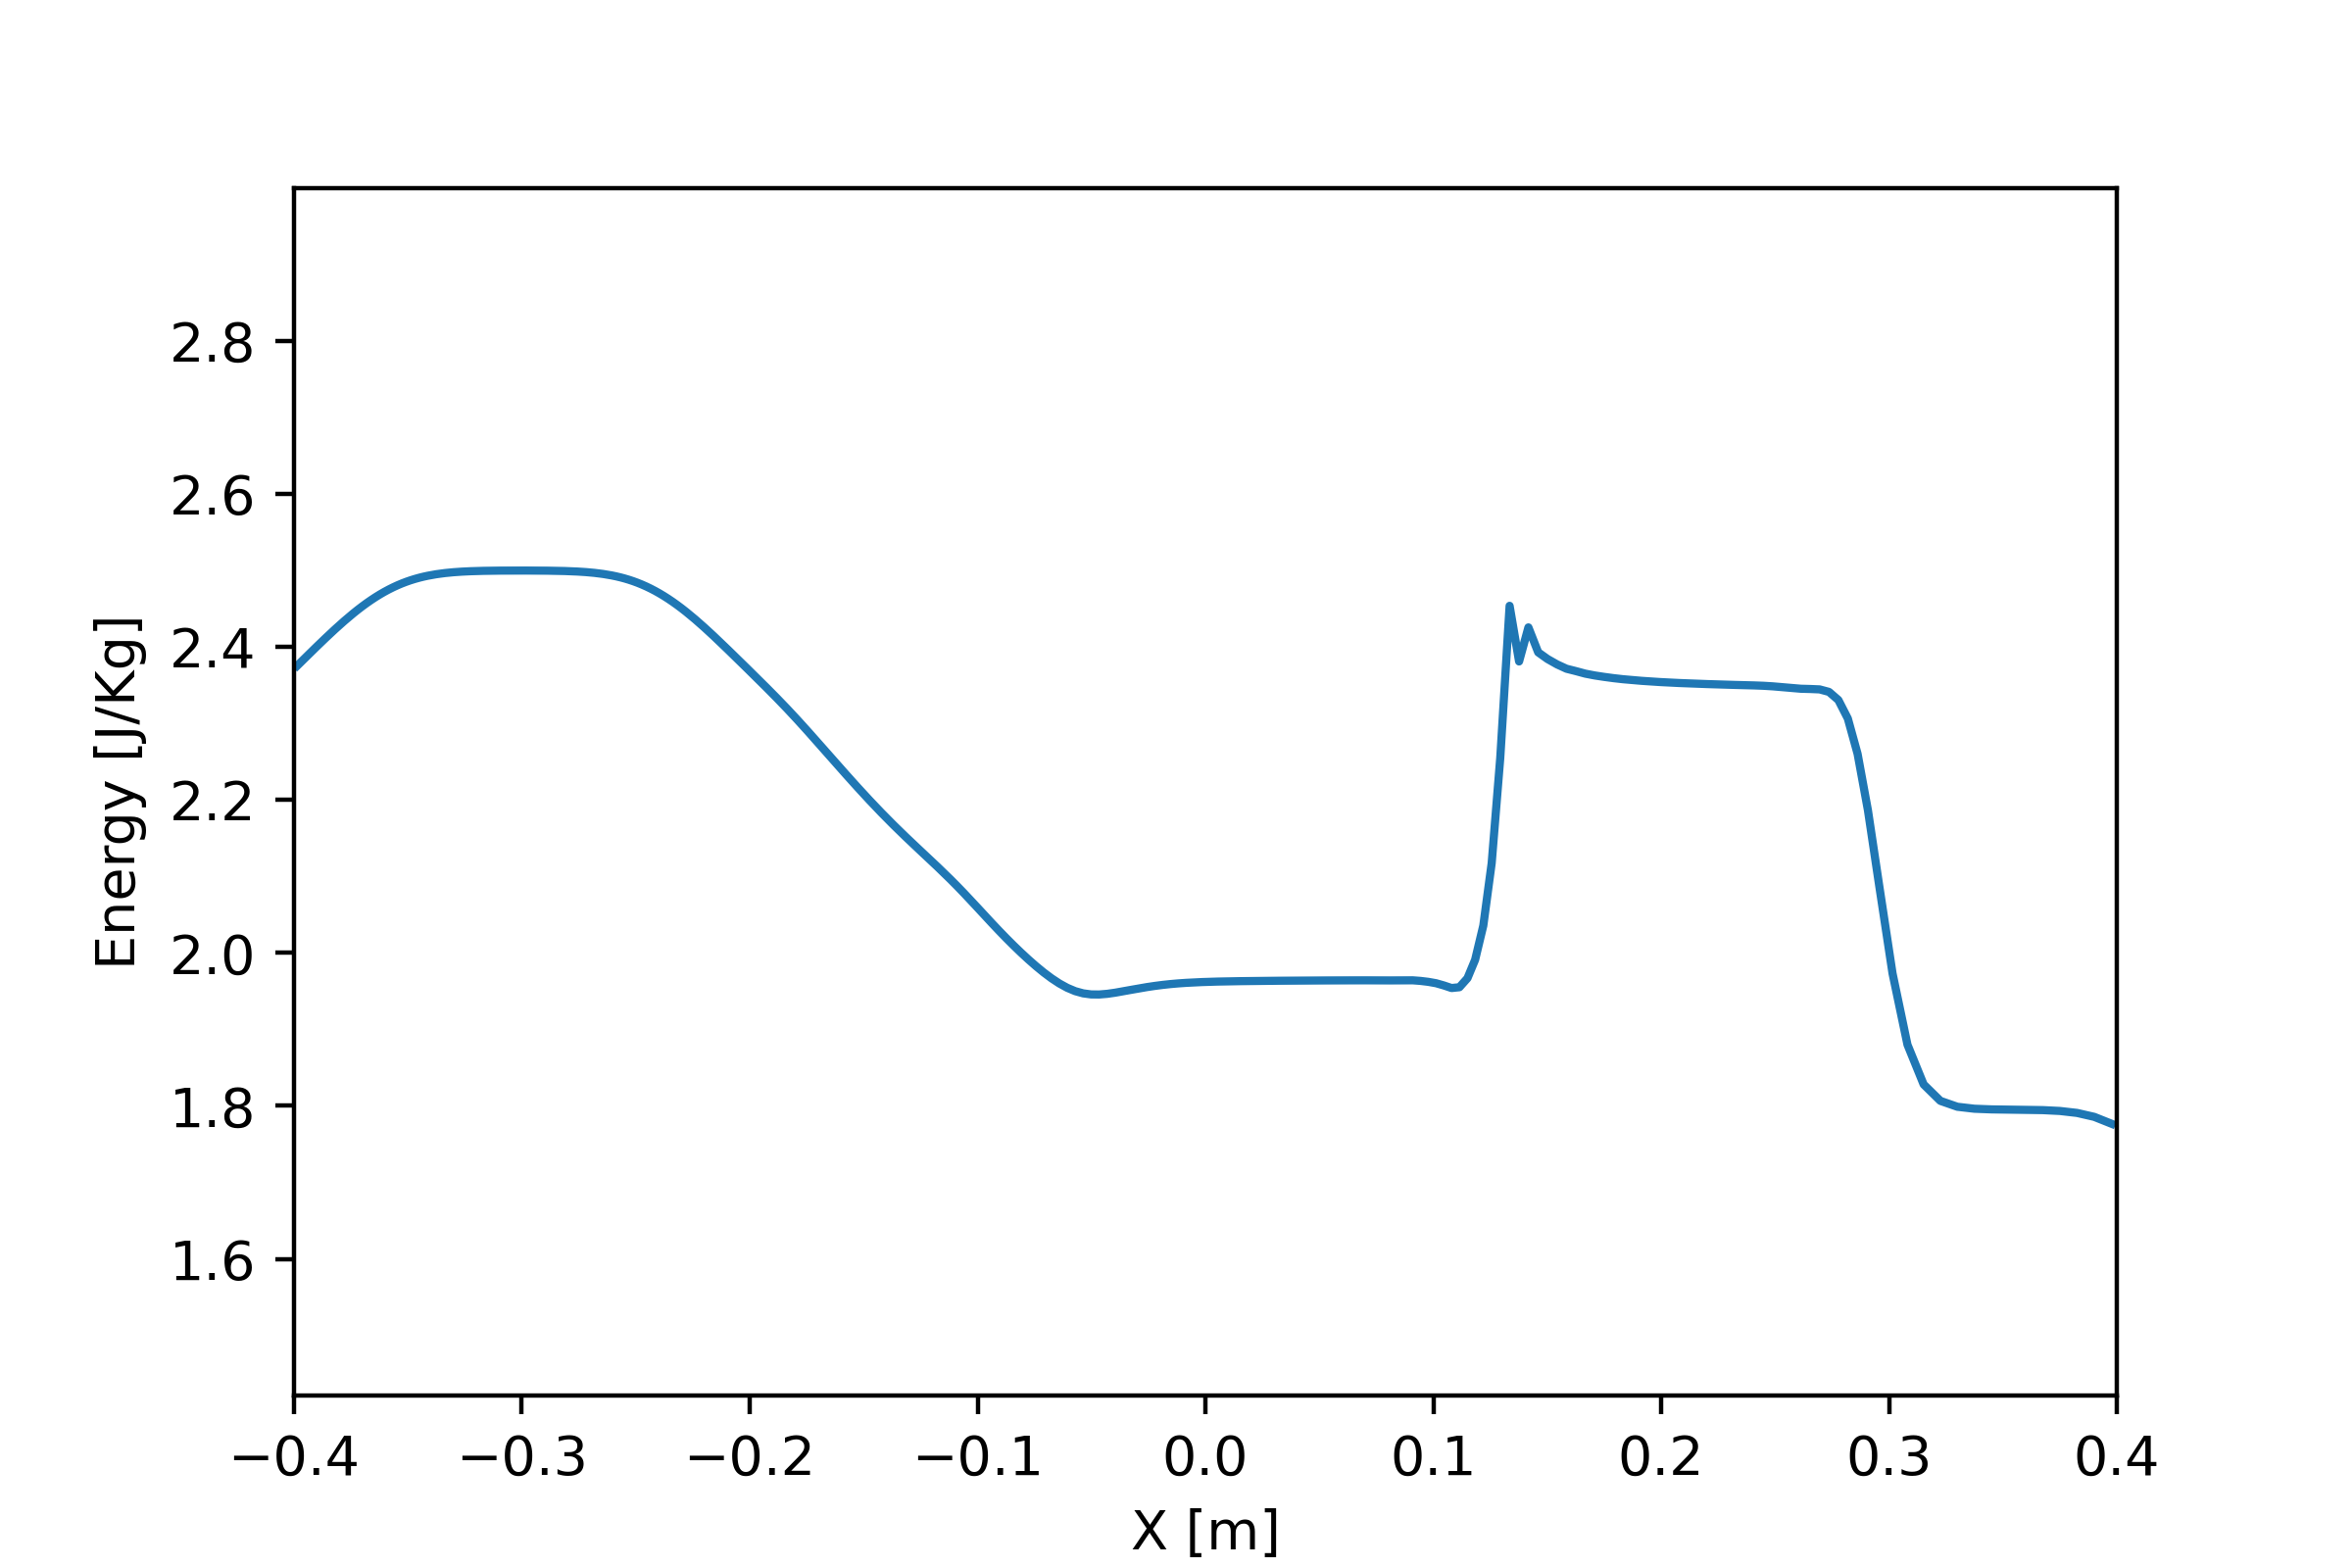
\includegraphics[width=\linewidth]{/home/andreas/Lund/FYSN33/Labs/SPH/SPH-Lab/1D/Energy.png}
	\end{subfigure}
	\hfill
	% Bottom-right
	\begin{subfigure}[c]{0.45\textwidth}
		\centering
		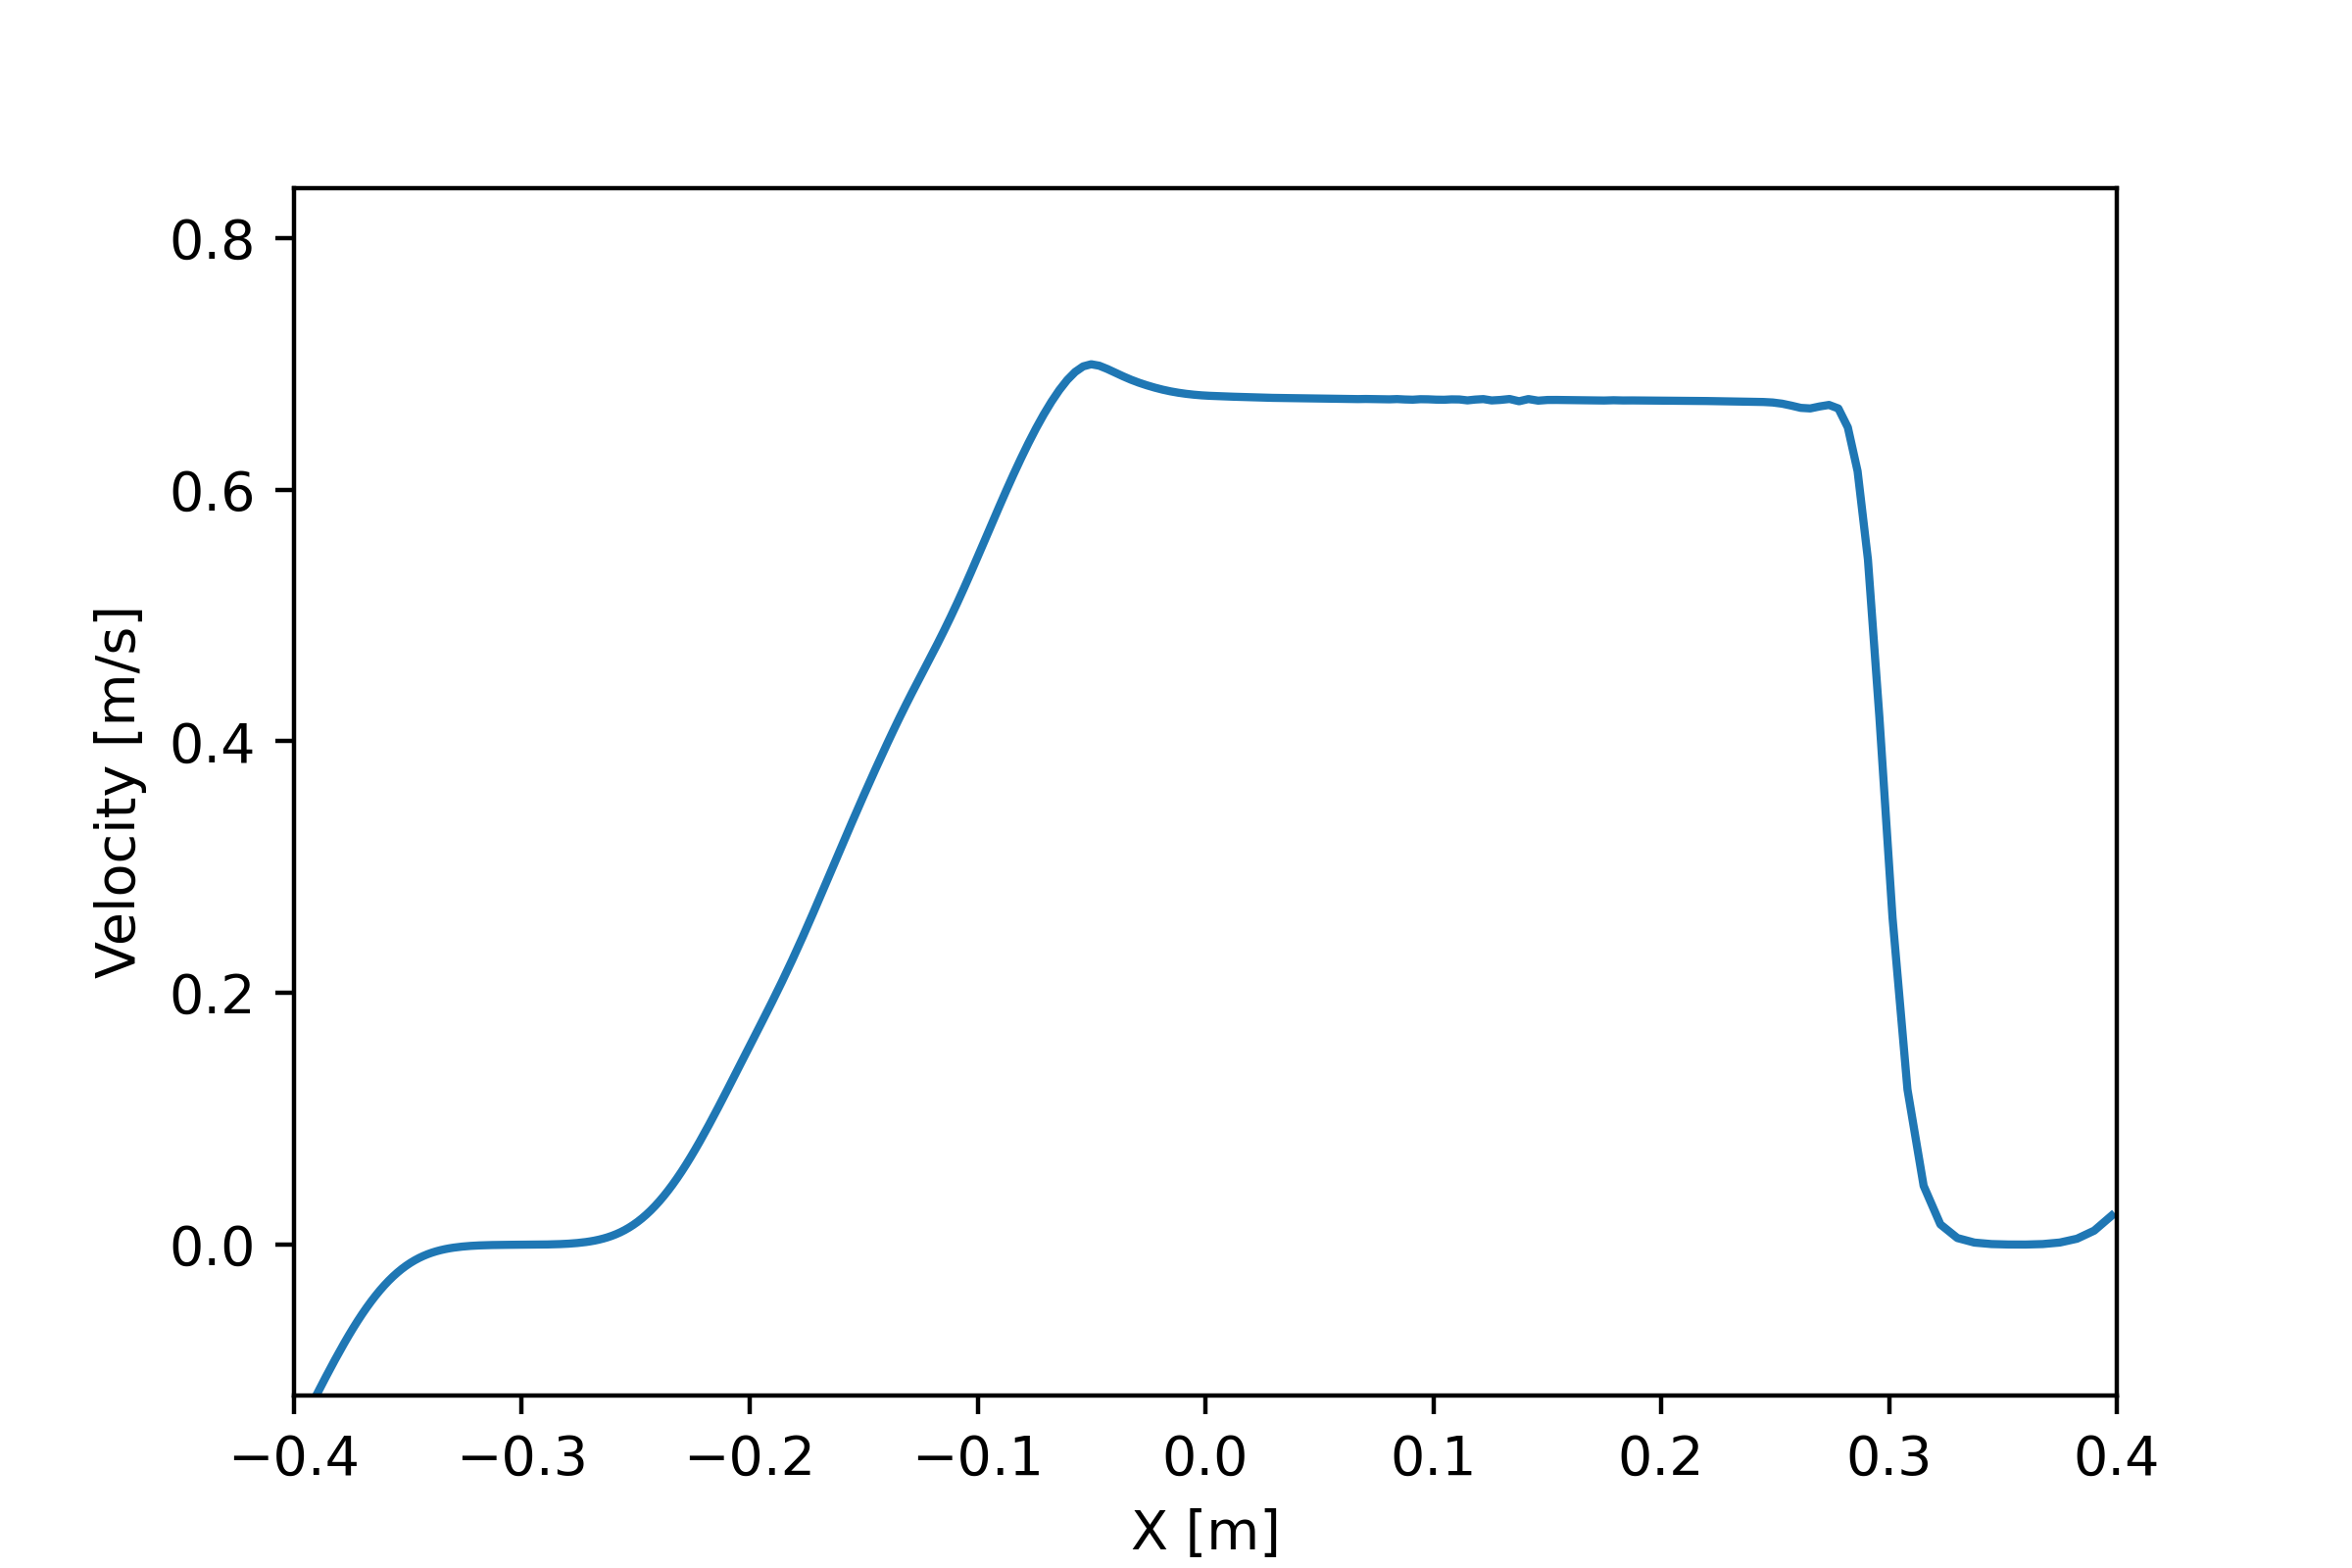
\includegraphics[width=\linewidth]{/home/andreas/Lund/FYSN33/Labs/SPH/SPH-Lab/1D/Velocity.png}
	\end{subfigure}
	
	\caption{Density, pressure, internal energy and velocity of the system versus the $ x $-coordinate.}
	\label{fig:1d}
\end{figure}

The results are close to the expected values from previous simulations from the lab manual\cite{Hobbs}. 

\subsection{Planet Collision}

Unfortunately, the produced simulation for the planetary collision didn't work as expected. Although movement is produced, the planets collide and result in a spike in pressure, causing most particles to gain immense velocities and escape the planet formations.

\section{Conclusion}

The 1-D Sod's shock tube part of the project shows almost exact comparison to the expected values. We conclude that the method implemented does what it should at an acceptable level. Furthermore, the time for simulation is gratifying, w

The planetary collision problem would have required more time for solving bugs in the code. We were able to produce moving particles in a 3-D environment. However it seems that gravitation, although implemented, didn't work as expected, and that the term \textbf{REF} was large in comparison. More time would be needed to debug this issue.

\newpage
\addcontentsline{toc}{section}{References}
\printbibliography

\end{document}